% Created 2020-12-16 Wed 21:00
% Intended LaTeX compiler: pdflatex
\documentclass[11pt]{article}
\usepackage[utf8]{inputenc}
\usepackage[T1]{fontenc}
\usepackage{graphicx}
\usepackage{grffile}
\usepackage{longtable}
\usepackage{wrapfig}
\usepackage{rotating}
\usepackage[normalem]{ulem}
\usepackage{amsmath}
\usepackage{textcomp}
\usepackage{amssymb}
\usepackage{capt-of}
\usepackage{hyperref}
\usepackage[margin=0.8in]{geometry}
\usepackage{amssymb,amsmath}
\usepackage{graphicx}
\documentclass[12pt]{article}
\usepackage{hyperref}
\usepackage{multicol}
\usepackage[T1]{fontenc}
\usepackage[utf8]{inputenc}
\graphicspath{{.}}
\usepackage{cite}
\author{Andrea Malleo and Reggie Gomez}
\date{\today}
\title{Occupancy Networks: NYU Computer Vision Fall 2020 Final Project}
\hypersetup{
 pdfauthor={Andrea Malleo and Reggie Gomez},
 pdftitle={Occupancy Networks: NYU Computer Vision Fall 2020 Final Project},
 pdfkeywords={},
 pdfsubject={},
 pdfcreator={Emacs 26.3 (Org mode 9.4)}, 
 pdflang={English}}
\begin{document}

\maketitle
\section{Introduction}

\begin{multicols}{2}
  We present an implementation of an existing technique for 3D reconstruction via the learned approximation of surface boundaries. Specifically we followed the method presented in Occupancy Networks \hyperlink{ref1}{1} to train a neural network classifier to learn the continuous decision boundary representing the implicit surface of some class of objects. The network maps coordinates in 3D space to a value between 0 and 1, representing the probability that point lies inside an instance of a 3D mesh. This mesh generation inference process is either conditioned on images of an object, or unconditioned, decoding from a latent variable sampled from the learned distribution of an encoding in 3d mesh function space. The resulting meshes generated produce a continuous distribution of instances within the category the model was trained on.
  \par
  \\
  A learned model for 3D representation sits a layer above existing methods for storing 3D representations such as point clouds, voxels, and meshes, in that the model can generate countless instances of all three. The trained Occupancy Network evaluates at any point whether or not that point lies within a mesh. It can be evaluated on a grid of points of arbitrary resolution and exhibits generative capabilities on an entire category of objects. From a set of coordinates and their occupancy values, point clouds can be extracted directly, namely by taking all of the coordinates with an occupancy probability over a certain threshold. See \hyperlink{fig1}{Figure 1}. For the actual mesh representation, further computation is necessary. Specifically, inputting the points and their occupancies into the Marching Cubes algorithm will produce meshes such as the one in \hyperlink{fig5}{Figure 5}.

  \\
  The Occupancy Networks paper came out as one of a small batch of papers in 2019 all showcasing similar work learning implicit fields for generative shape modeling. In \hyperlink{ref4}{Park et al.} not just a binary classification but a continuous signed distance function is learned. This network takes an input 3D coordinate and returns a number indicating the magnitude of the distance between this coordinate and the surface of the mesh, and a sign indicating if that point lies inside (negative) or outside (positive). On the unconditional generation side, OccupancyNetworks \hyperlink{ref1}{1}, and us in their footsteps, use a variational auto-encoder to learn the mean and standard deviation of Gaussian distribution on a 128 dimension latent vector representing instances of a mesh in some class, whereas \hyperlink{ref4}{4} formulates their own auto-decoder that sidesteps the need for an encoder component in the model architecture. Deep Level Sets \hyperlink{ref5}{5} and Learning Implicit Fields for Generative Modeling \hyperlink{ref6}{6} also present networks that produce inferred 3D shapes exhibiting smoothness, continuity, and detail not found in their recent forerunners.

  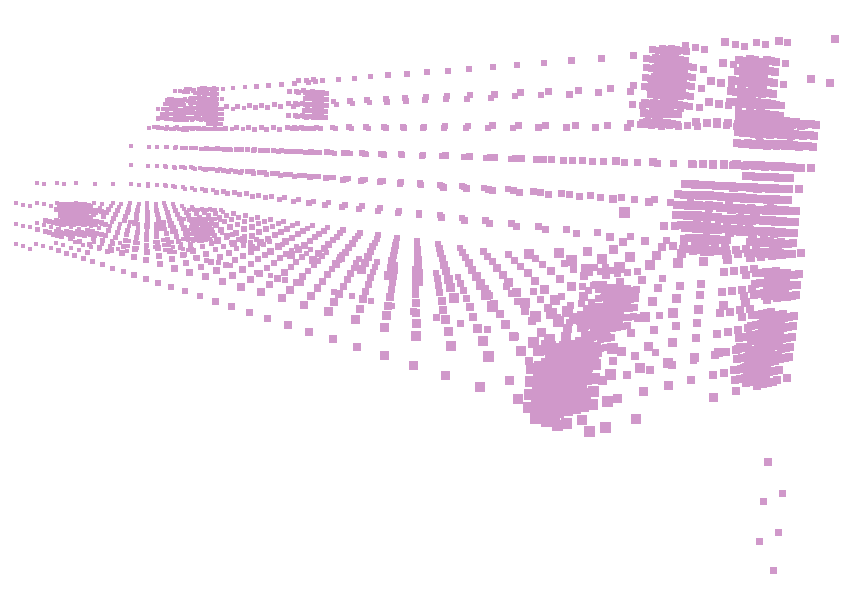
\includegraphics[scale=0.3]{./benchImages/bench_pointcloud.png} \\
  \caption{\hypertarget{fig1}{\textbf{Figure 1}} This point cloud was generated by evaluating our Occupancy Network trained on the bench mesh data set and setting the threshold for occupancy as a probability greater than or equal to 0.1.


    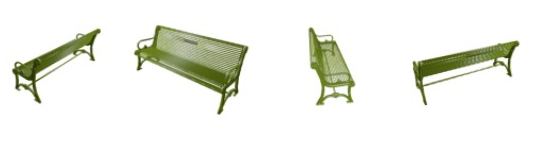
\includegraphics[scale=0.6]{sampleTrainingBench/benches.png}
    \catption{\hypertarget{fig2}{\textbf{Figure 2}} These four images are examples of the input used to train our network. Here is a single instance of a bench, pictured from random orientations. At training time, one of these would be randomly selected to condition a set of points sampled over a grid containing this mesh with their ground truth occupancy values.}

    \section{Method}
    In this section we discuss the source and preprocessing of the training data. Then we outline the goals of the three experiments we conducted and compare and contrast the model architectures and training times. Finally we touch on the inference process, and the follow up steps for visualizing the resultant meshes.

    The dataset used to train all the models was downloaded preprocessed from the authors of Occupancy Network off \hyperlink{ref3}{Github}. The data is from the \hyperlink{ref2}{ShapeNet} dataset and for each category of shapes (chair, bench, phone, cabinet, sofa) there are hundreds of instances of such an object, each of which has thirteen still images taken from different orientations. See \hyperlink{fig2}{Figure 2}. Additionally, for each mesh instance, there are 100,000 coordinates from uniform sampling of the unit cube centered at (0,0,0). For each of the points there is a corresponding ground truth occupancy value in $\{0,1\}$. The preprocessing steps that we did not repeat include filtering out non-water tight meshes from the original dataset, and running the algorithm that determines this ground truth for each coordinate. \\


    \subsection{Training}
    All model architectures we produced \footnote{https://github.com/reggieag/nyu\_occupancy\_networks\_project} emulate those used in the paper. Where any component was unclear from the description and images of the paper, we consulted the available \hyperlink{ref3}{implementation}. This step was limited to debugging. All three experiments share a common pipeline that the coordinates are passed through. They all differ in their means of computing an encoding on which to condition the training. The encoding is either from a 2d image tensor, or simply from the points themselves.
    \par
    \\
    Experiment one concerns the generation of meshes conditioned on a still image of an instance of the input category.  The input to each 'mini-batch' consisted of a single image, randomly drawn from the thirteen available for each instance and some $K$ coordinate points from the ground truth of that mesh. The image went into an encoder block, which in this case was a downloaded ResNet-18 architecture pretrained on the ImageNet dataset \hyperlink{ref2}{2}. The output of the encoder is passed into a fully-connected layer to project the features to a 256 dimension encoding $c$. The points meanwhile are essentially passed through five \hyperlink{ref7}{ResNet} blocks. Crucially, the conditional batch normalization
    \begin{flalign*}
      x_{out} = \gamma(c)b + \beta(c)\\
    \end{flalign} is computed twice inside of each ResNet block where
    \begin{flalign*}
      b &= \frac{x_{in}-\mu}{\sqrt(\sigma^2 + \epsilon)}\\
    \end{flalign*}
    is the BatchNorm1d with affine set to False and running mean and variance stats are tracked and used by Pytorch.
    Note that each time conditional batch normalization is performed, $c$, computed once, is passed through two disjoint fully connected layer heads to generate the backprop refined $\beta$ and $\gamma$ vectors. The loss function used during training is cross entropy classification loss averaged over all points across all minibatches. Let $B$ denote the batch size and $K$ the number of points for each instance or minibatch.
    \begin{flalign*}
      L(\theta, \psi) &= \frac{1}{B*K} \sum_{i=1}^{B} \sum_{k=1}^K L(f_{\theta}((p_{ij},z_{ij}),o_{ij}))
    \end{flalign}
    \\
    \par
    Training for this experiment lasted over day, which is an outlier from the next two experiments, due to all of the images pumped in per batch.
    \par
    Experiment two sought to reconstruct noisy and incomplete point clouds. The conditioning step here comes from the output of a PointNetEncoder \hyperlink{ref10}{10}. The PointNet encoder has 4 basic ResNet blocks and two fully connected layers. Between the blocks there is max pooling and expansion. The output is projected to a 512 dimensional vector encoding, which is the $c$ input to the conditional batch normalization step. The loss function is identical to the above.
    \par
    Experiment three involved learning a probabilistic latent variable model for representing the mesh function space. This model just takes points and occupancies, and first passes the points in to an \hyperlink{ref8}{AutoVariational Encoder} module. The architecture of this network is a slight variation on the Point Cloud Completion encoder just described, the most significant difference being that the output are two vectors for the mean $\mu_{\psi}$ and log-standard deviation $log(\sigma_{\psi}^2)$ of a 128 dimensional latent code z. In each forward pass, once these two vectors are computed, a sample from this distribution is drawn as $(e^{\sigma_{\psi}}*rand()+ \mu_{\psi})$. This 128 dimensional vector is now an encoding, and used like in experiment one for the conditional batch normalization. The loss function here is two pronged, composed of both the binary cross entropy loss between the computed probablities and the target occupancies, and the KL divergence of the generated $\mu_{\psi}$ and $\sigma_{\psi}$ from a Gaussian distribution of mean 0 and standard deviation 1. \hyperlink{ref8}{8} \begin{flalign*}
      L(\theta, \psi) &= \frac{1}{|B|} \sum_{i=1}^{|B|} \sum_{k=1}^K L(f_{\theta}((p_{ij},z_{ij}),o_{ij})) \\
      &+  \frac{-1}{2} \sum (1 + \sigma_{\psi} - \mu^2 - e^{\sigma_{\psi}} )
    \end{flalign}
    In this way the network is able to learn an encoding of mesh instances in a reduced dimension. The data from 100 3d coordinates can be efficiently represented in only 128 dimensions, which become a way to control generation of a mesh during the inference procedure.

    \subsection{Mesh Generation}\\
    \par
    The mesh generation procedure can be summarized as follows. The trained model takes a batch of coordinates in 3D space and either a single still image to condition the output (experiment 1), or a random variable drawn from the learned distribution (experiment 3). Because the network learns a continuous occupancy function, it can be evaluated at any resolution of points. The first idea might be to generate a set of coordinates that uniformly sample the 3d unit cube centered at (0,0,0) at the desired resolution. However, one of the drawbacks of existing 3D representations is the cubic memory demand of voxels. This approach would face the same pitfall were a naive uniform sampling scheme employed. Instead a more efficient grid is used, one that the Occupancy Network authors describe as the first step in their process of \textbf{Multiresolution IsoSurface Extraction}.
    \\
    \par
    We begin by evaluating the occupancy on a $32^3$ grid of voxels. Every coordinate on this grid is assigned a probability. We set a threshold value of 0.1 in experiment 1, and 0.3 in experiment 2, at or above which a point is given an occupancy value of 1, otherwise it is marked 0. Next for every voxel whose corner coordinates are a mix of occupied and unoccupied, this cube is divided into 8 subvoxels and reevaluated at all of its points. This process is repeated at most one more time, for a recursion depth of 2. In practice we have a grid that adapts to a finer grain resolution at the boundary of the mesh to allow for a more precise estimation of edges, not wasting memory by storing more than a coarse grid around the exterior of the mesh.
    \par
    \\
    Once we have a suitable set of coordinates written to one file, and their cooresponding occupancy values written to another, the next step is to apply the Marching Cubes algorithm \hyperlink{ref9}{9} to generate a set of triangles that compose the mesh. The Marching Cubes algorithm iterates over each voxel cube and considers the occupancy values at each corner. For each of the 256 permutations of possible patterns of occupancy (occupies or does not occupy for each of the 8 vertices), there are only about 15 unique cases (in the original publication). These are all tabulated in a map, and correspond to the set of triangles inferred from the estimated points of intersection. The union of all of the triangles found defines the mesh. The original algorithm has been refined and enhanced many times between its first publication and present day, however we only implemented the most basic, original one. See \hyperlink{fig3}{Figure 3} and \hyperlink{fig4}{4}. for the results of our MarchingCubes.
    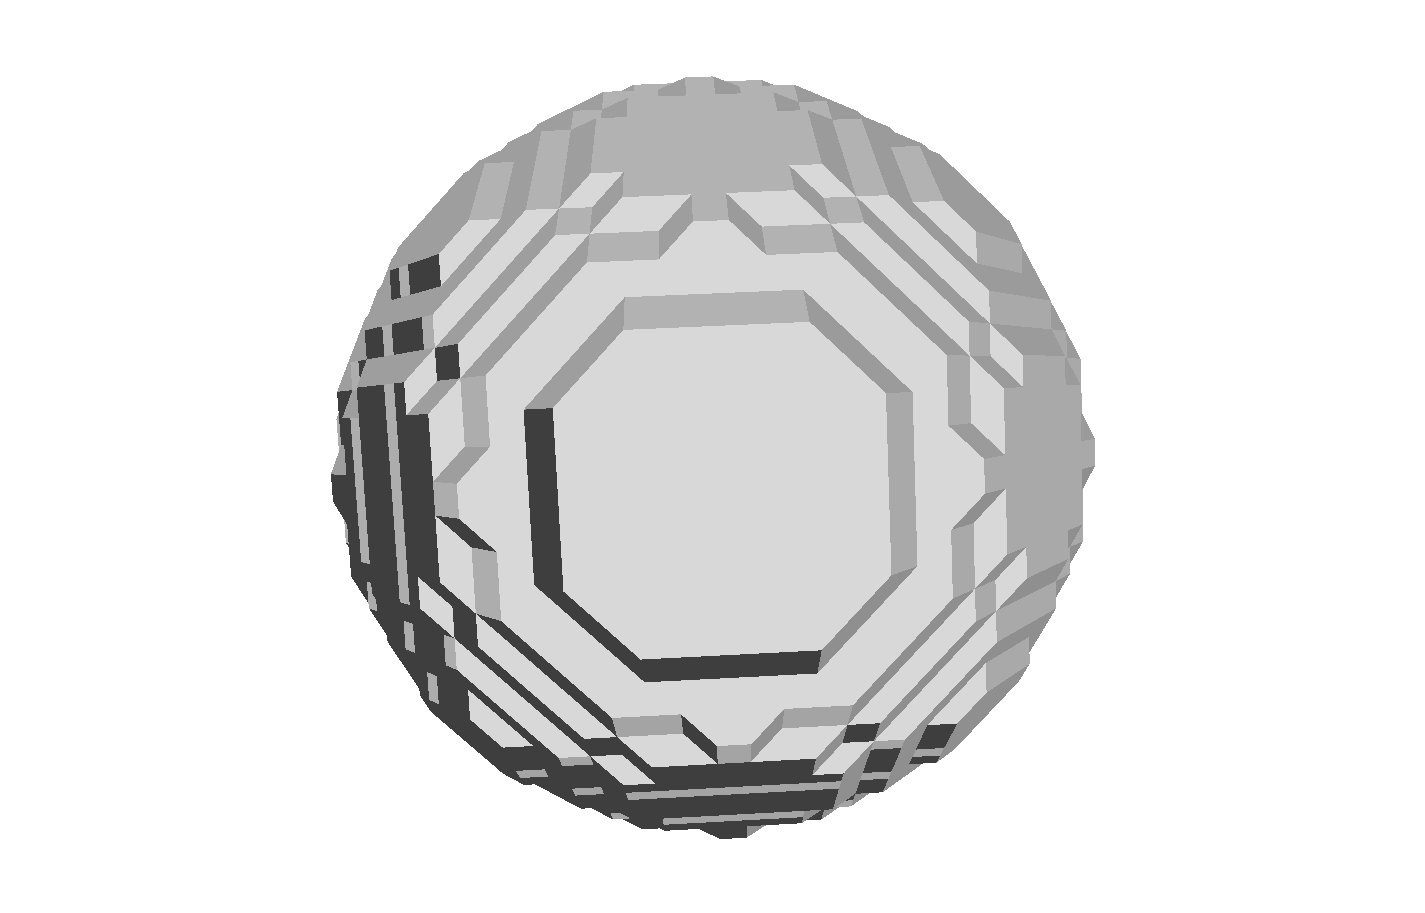
\includegraphics[scale=0.2]{MCImages/cubedUniformSnap.png} \\
    \caption{\hypertarget{fig3}{\textbf{Figure 3}} Here we rendered the implicitly defined sphere on a uniform $32^3$ voxel grid.}
    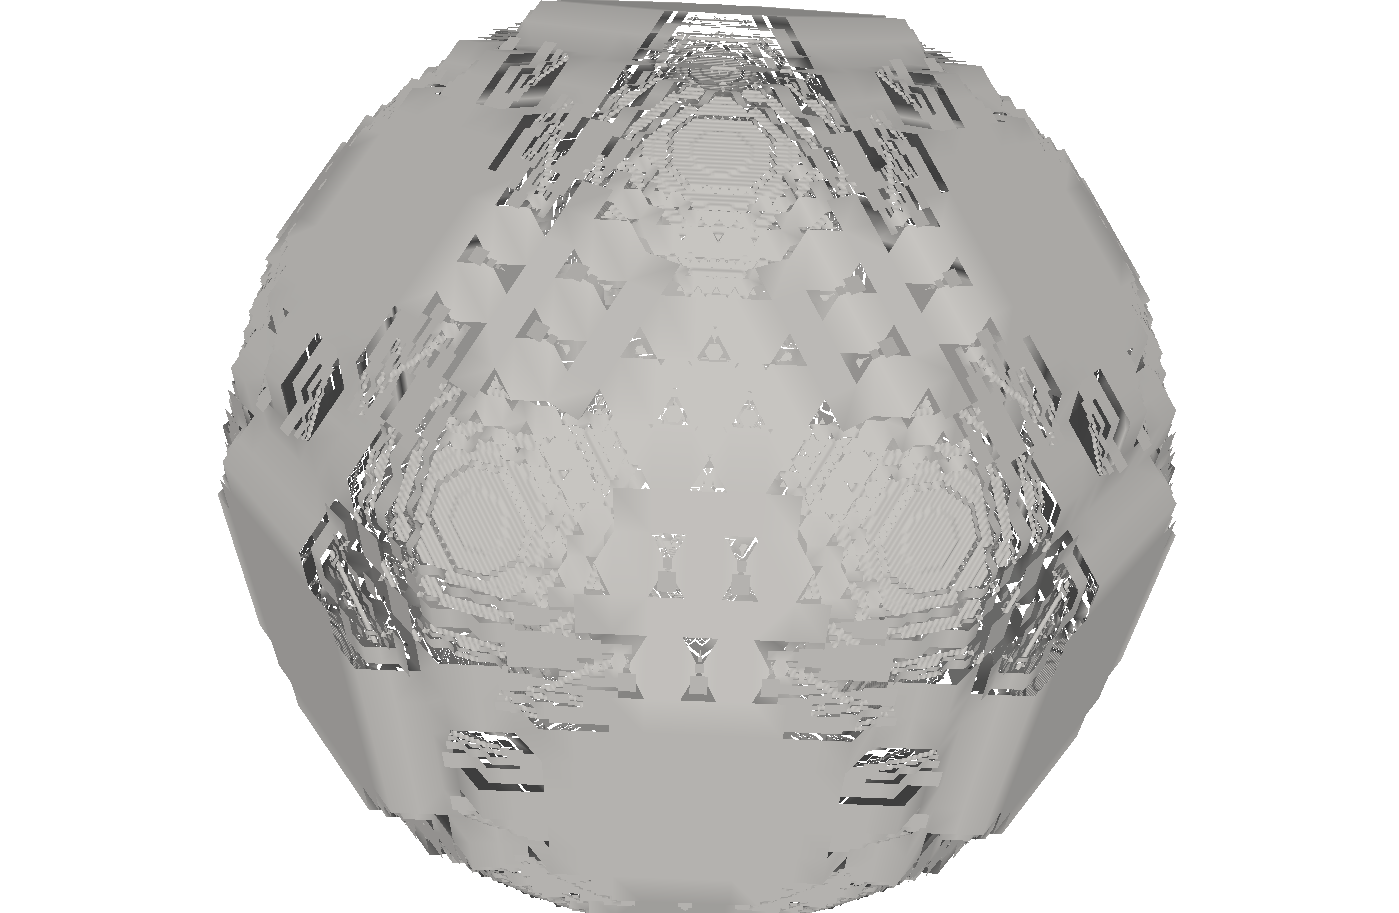
\includegraphics[scale=0.2]{MCImages/sphereAdaptiveSnap.png}\\
    \caption{\hypertarget{fig4}{\textbf{Figure 4}} Here we see the results for that same sphere when evaluated on an adaptive grid. Admittedly an unsatisfying result.}
    \\
    \par
    The .off files written by Marching Cubes can be visualized most simply with a 3rd party opensource application such as Meshlab. We did, however input these mesh files into a rasterizer written as part of the Computer Graphics class this semester and generated stills and gifs of the resultant meshes. Please go to our github page to see gifs. For experiment 1, please see the video that rotates around the generated bench mesh. For experiment 2, please see the video showing the phone mesh generated from an incomplete point cloud. For experiment 3, please see the video that illustrates interpolation in latent variable space, and the resulting continuous deformations to the couch mesh.


    \section{Experiments}

    \textbf{Experiment 1:} The goal of the first experiment was to train a model that achieves 3D mesh reconstruction from a single 2D image of the object from an arbitrary angle of view. In our case we trained on the bench category. We trained over nine epochs, and for this network that took over a day. At inference time, we randomly draw one of the thirteen images from different orientations to condition the evaluation on. The results are illustrated in \hyperlink{fig5}{Figure 5}. The mesh is recognizably a bench, but is not a closed mesh. A collection of the results from the original paper are presented in Figure 8. It must be noted that a critical difference between our rendering process and the original authors, is that they go on to run their mesh through two optimizations, one to reduce the number of faces, and a second that minimizes the difference between the normals on the computed mesh with the gradient information on the points collected by backpropping the network. We performed neither of these steps. Still, a clear continuation of this work would be to improve the performance of this rendering. From \hyperlink{fig4}{Figure 4} it is clear that the current Marching Cubes implementation does not succeed fully on an adaptive grid. It is our belief that it is chiefly responsible for the slated mesh seen in Figure 5, since the validation scores on this network were $99\%$.

\end{multicols}

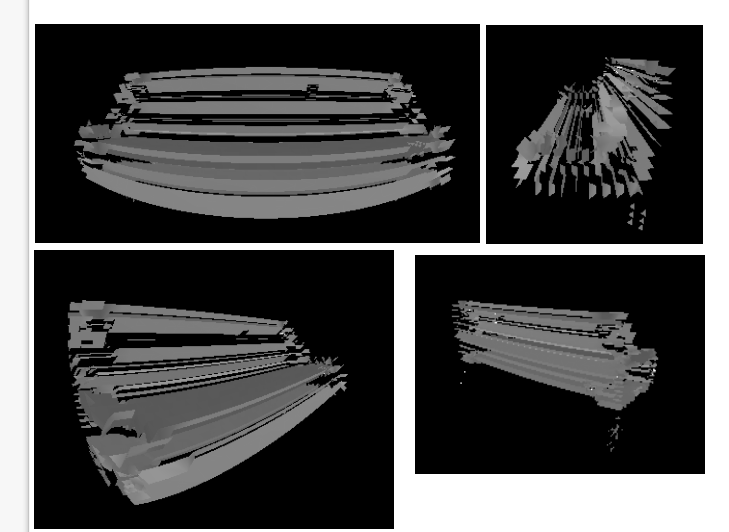
\includegraphics[scale=0.6]{benchImages/benches.png} \\
\caption{\hypertarget{fig5}{\textbf{Figure 5}} Results from the Single Image Reconstruction experiment. Here is one instance of a bench mesh viewed from a variety of angles.}\\
\\

\textbf{Experiment 2:}
The goal of the second experiment was to train a model that achieves 3D mesh reconstruction, but with a noisy point cloud passed in at inference instead of a single 2D image like in experiment 1. Our model was trained on the phone category for one epoch. At inference time, we randomly chose 300 points out of 100,000 from the complete point cloud representation. We then passed those 300 sampled points to a PointNet encoder. The PointNet encoder then feeds into the Occupancy Network the same as in experiment 1. We found that the model was able to train fairly accurately within one epoch. Accuracy was around 99\% when we ran validation on the model. If you look at Figure 6 you can see some rendered results. You can see that the body of the phone was learned fairly well, but the model was not able to recognize the antenna. One possible extension would be to render a denser point cloud from the trained occupancy network.

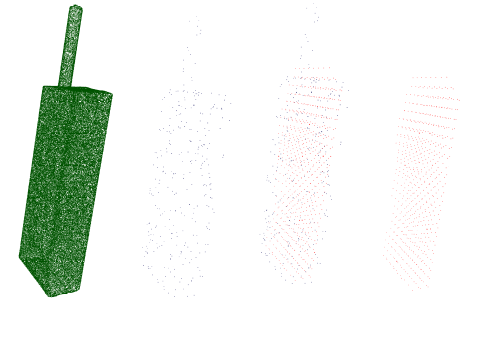
\includegraphics[scale=1.4]{phoneImages/compilation.png} \\
\caption{\hypertarget{fig6}{\textbf{Figure 6}} Here we have 4 images showing respectively a) The ground truth point cloud of a phone from the data set. b) the incomplete point cloud input at inference time. c) the completed point cloud containing the predicted and provided coordinates. d) just the predicted points produced by the Point Completion network}\\

\textbf{Experiment 3:} The goal of the second experiment was to learn a distribution over a latent embedding of the mesh category for unconditioned generation of 3d meshes and demonstrate the continuous nature of this distribution by interpolating in the latent space. \hyperlink{fig7}{Figure 7} depicts a couch mesh produced from a random z. From experiments during inference, we found the bounds of the z to indeed approach that in a distribution with standard deviation of 1. Given a z vector composed of values of magnitude 5 or greater, the network produced an empty grid. The probability threshold required more attention to here as compared to experiment 1. We needed to raise it in order to filter out couches with inflated bases. The gif posted on our Github page provides the best demonstration of our results.



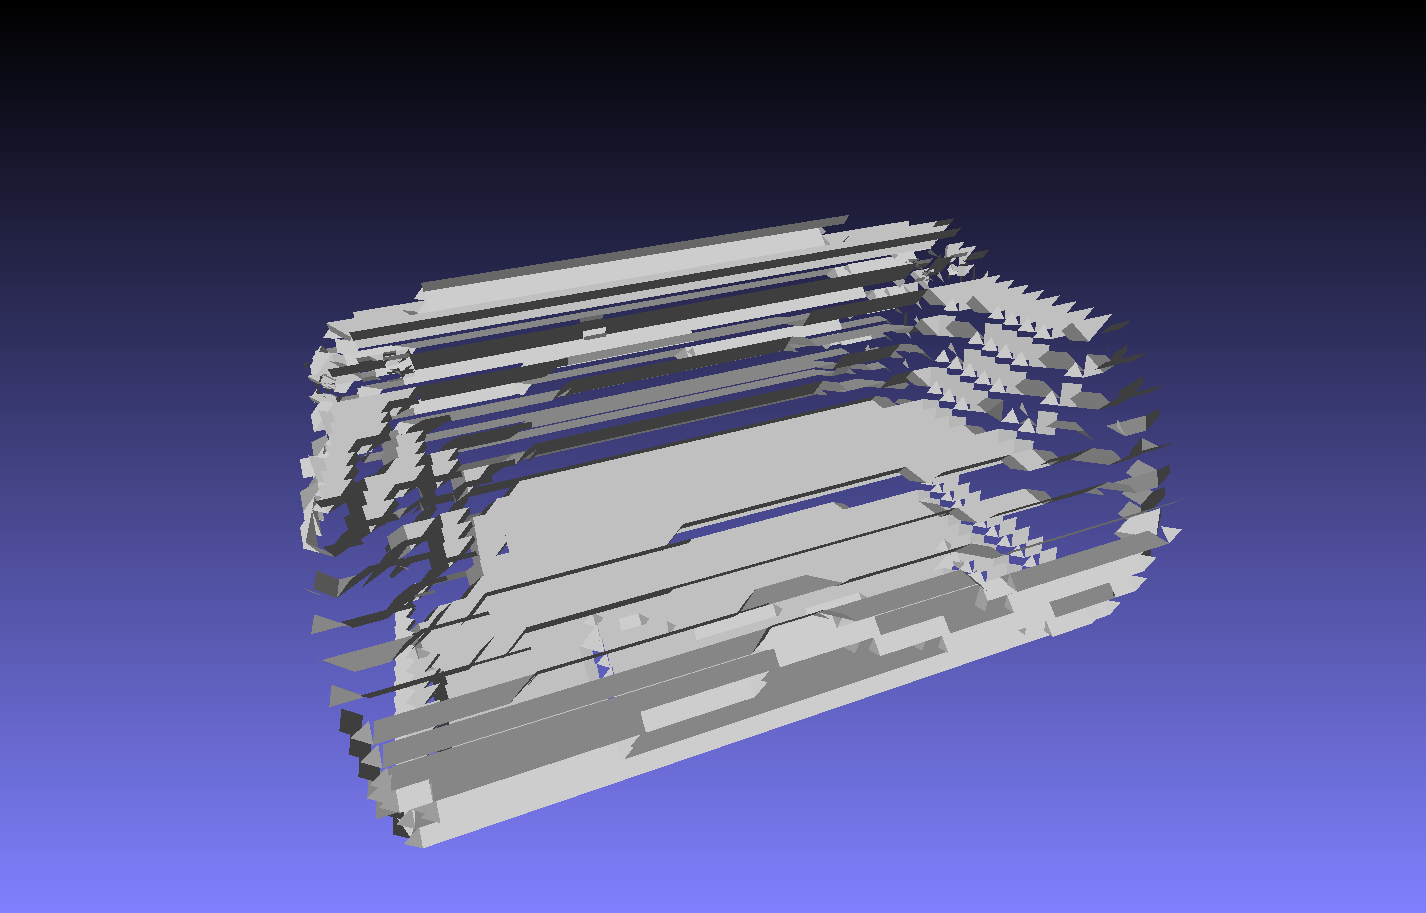
\includegraphics[scale=0.4]{./benchImages/couch.png}\\
\caption{\hypertarget{fig7}{\textbf{Figure 7}} A Meshlab rendering of one randomly generated couch mesh. Note the varying size of solid pieces, particularly on the arm rest area of the couch. This is evidence of the MultiResolution technique, where the resolution of the image increases at the boundary of the mesh. }

\section{Discussion}
\begin{wrapfigure}{l}{}
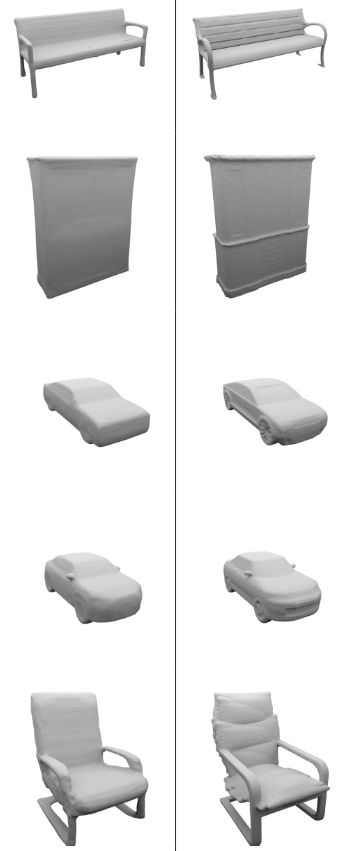
\includegraphics[scale=0.4]{./benchImages/groundTruth.png}
\end{wrapfigure}

In this paper, we documented our journey reproducing the existing concept of Occupancy Networks as an expressive and efficient representation for 3D meshes. We performed three experiments that tested the capability of our models to generate meshes conditioned on an input image, reconstructed from an incomplete and noisy point cloud, and from a latent variable in mesh function space. In all three cases we were able to demonstrate the ability to generate such meshes on the bench, phone, and sofa object categories respectively. While the rendering results of our homespun Marching Cubes implementation leave a clear direction of future work, there are more next steps to be done on the learning side. The space of suitable conditioning inputs has not been fully explored, for instance with real-life photos of chairs for experiment 1. Additionally, a clear representation of the different manifestations of couch meshes on the perimeter of the latent space would be enlightening to investigate. \\

\textbf{Figure 8 from \hyperlink{ref1}{1}} In the left column, the authors present their resulting meshes for a variety of object classes, and on the right column is the respective ground truth mesh.

\clearpage

\section{References}
\begin{enumerate*}
\item \hypertarget{ref1}{[1]}  Lars and Oechsle, Michael and Niemeyer, Michael and Nowozin, Sebastian and Geiger, Andreas. Occupancy Networks: Learning 3D Reconstruction in Function Space Mescheder, In Proc IEEE Conf. on Computer Vision and Pattern Recognition (CVPR).2019
\item \hypertarget{ref2}{[2]} J. Deng, W. Dong, R. Socher, L. jia Li, K. Li, and L. Fei-fei.  Imagenet:  A large-scale hierarchical image database.  InProc. IEEEConf. on Computer Vision and Pattern Recognition (CVPR), 2009.
\item \hypertarget{ref3}{[3]} https://github.com/autonomousvision/occupancy\_networks
\item \hypertarget{ref4}{[4]} Jeong Joon Park and Peter Florence and Julian Straub and Richard Newcombe and Steven Lovegrove. DeepSDF: Learning Continuous Signed Distance Functions for Shape Representation. arXiv:1901.05103. 2019
\item \hypertarget{ref5}{[5]} Mateusz Michalkiewicz and Jhony K. Pontes and Dominic Jack and Mahsa Baktashmotlagh and Anders Eriksson. Deep Level Sets: Implicit Surface Representations for 3D Shape Inference. arXiv:1901.06802. 2019
\item \hypertarget{ref6}{[6]} Zhiqin Chen and Hao Zhang. Learning Implicit Fields for Generative Shape Modeling. arXiv:1812.02822. 2019.
\item \hypertarget{ref7}{[7]}Kaiming He, Zhang,Ren, Sun. Deep Residual Learning for Image Recognition. arXiv:1512.03385.  2015
\item \hypertarget{ref8}{[8]} https://github.com/geyang/variational\_autoencoder\_pytorch
\item \hypertarget{ref9}{[9]} Lorenson and Cline. Marching Cubes: A High Resolution 3D Surface Construction Algorithm. Computer Graphics Volume 21, Number 4, 1987.
\item \hypertarget{ref10}{[10]} H. Fan, H. Su, and L. J. Guibas.  A point set generation network for 3D object reconstruction from a single image.  InProc. IEEEConf. on Computer Vision and Pattern Recognition (CVPR), 2017
\end{enumerate}
\end{document}
